\documentclass{standalone}
% Author: Carl Richard Theodor Schneider
\usepackage{tikz}

\usetikzlibrary{calc,positioning}

\begin{document}
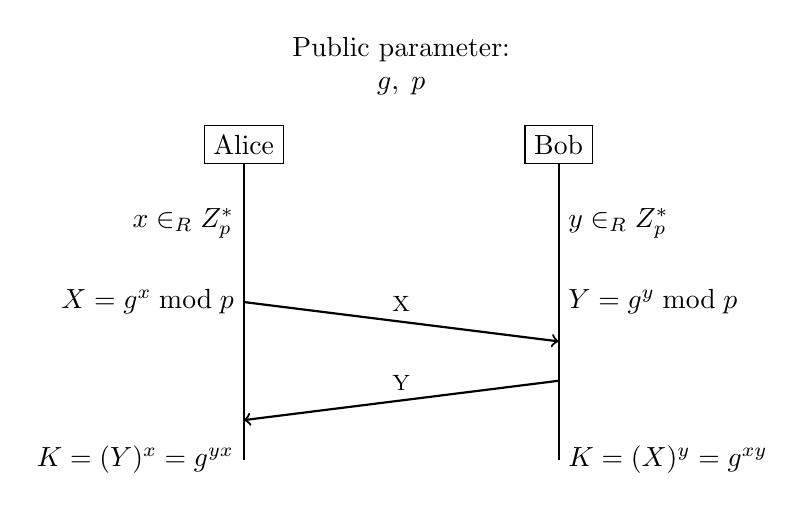
\begin{tikzpicture}
  % Public parameter:
  \node[draw=none,fill=none,align=center] (public) at (0,1) {Public parameter:\\$g,\; p$};
  
  % Alice
  \node[draw] (Alice) at (-2,0) {Alice}; 
  \draw[thick] (Alice) -- ++(0, -4);
    
  % Calculations of Alice
  \node[draw=none,fill=none,anchor=east] (asecret) at ($(Alice) + (0,-1)$) {$x \in_{R} Z_p^*$};
  \node[draw=none,fill=none,anchor=east] (Apublic) at ($(Alice) + (0,-2)$) {$X = g^{x} \bmod{p}$};
  \node[draw=none,fill=none,anchor=east] (akey) at ($(Alice) + (0,-4)$) {$K = (Y)^{x} = g^{yx}$};
    
  % Bob
  \node[draw] (Bob) at (2,0) {Bob}; 
  \draw[thick] (Bob) -- ++(0, -4);
   
  % Calculations of Bob
  \node[draw=none,fill=none,anchor=west] (bsecret) at ($(Bob) + (0,-1)$) {$y \in_{R} Z_p^*$};
  \node[draw=none,fill=none,anchor=west] (Bpublic) at ($(Bob) + (0,-2)$) {$Y = g^{y} \bmod{p}$};
  \node[draw=none,fill=none,anchor=west] (bkey) at ($(Bob) + (0,-4)$) {$K = (X)^{y} = g^{xy}$};
   
  % Messages
  \draw[->,thick] ($(Alice)+(0,-2)$) -- ($(Bob)+(0,-2.5)$) node [pos=0.5,above,font=\footnotesize] {X};
  \draw[->,thick] ($(Bob)+(0,-3)$) -- ($(Alice)+(0,-3.5)$) node [pos=0.5,above,font=\footnotesize] {Y};
    
\end{tikzpicture}
\end{document}
